% !TeX program = lualatex
\documentclass[fontsize=11bp]{article}

\usepackage{scrextend}
\usepackage[english]{babel}
%\usepackage{textcomp}
\usepackage{mathtools,amssymb,amsthm}
\usepackage[hmargin=1.25in,vmargin=1in]{geometry}
\usepackage{graphicx,cancel}
\usepackage{enumitem}
%\usepackage{unicode-math}
%\usepackage{mathpazo}
%\usepackage{mathptmx}
%\usepackage{helvet}

\usepackage[no-math]{fontspec}
\setmainfont{Times New Roman}[Ligatures=Rare]
\setsansfont{Arial}
\setmonofont{Courier New}
\let\hbar\relax
%\setmathfont[math-style=ISO]{Cambria Math}
\usepackage[lite,subscriptcorrection,nofontinfo]{mtpro2}
%\usepackage[integrals]{wasysym}
\usepackage{microtype}
\usepackage[colorlinks=true,allcolors=blue]{hyperref}
\usepackage{blindtext}
\usepackage{setspace}
\setstretch{1.132575757575758}
\setlength{\parindent}{18bp} %{.35in}
%\newcommand*{\bpsize}{\fontsize{11bp}{13bp}\selectfont}
%\AtBeginDocument{\bpsize}

\newcommand*{\parasp}{\setlength{\parskip}{10bp plus 2bp minus 3bp}}
\newcommand*{\noparasp}{\setlength{\parskip}{0bp plus 1bp}}
\newcommand*{\setparasp}[1]{\setlength{\parskip}{#1}}
\newcommand*{\pskip}{\vskip 10bp plus 2bp minus 3bp}
%\renewcommand{\CancelColor}{\color{red}}
%\newcommand*{\tcwm}{\textcompwordmark}
\parasp

\usepackage{titlesec}
\titleformat*{\section}{\sffamily\fontsize{11bp}{13bp}\bfseries\selectfont}
%\titleformat*{\section}{\sffamily\fontsize{14.4bp}{18bp}\bfseries\selectfont}
%\titleformat*{\subsection}{\sffamily\fontsize{12bp}{14bp}\bfseries\selectfont}
%\titleformat*{\subsubsection}{\sffamily\fontsize{11bp}{13bp}\bfseries\selectfont}
\titlespacing*\section{0pt}{3.25ex plus 1ex minus .2ex}{1.5ex plus .2ex -\parskip}
%\titlespacing*\section{0pt}{3.5ex plus 1ex minus .2ex}{2.3ex plus .2ex -\parskip}
%\titlespacing*\subsection{0pt}{3.25ex plus 1ex minus .2ex}{1.5ex plus .2ex -\parskip}
%\titlespacing*\subsubsection{0pt}{3.25ex plus 1ex minus .2ex}{1.5ex plus .2ex -\parskip}

\usepackage{ifthen}
\ifthenelse{\isundefined{\LEFTRIGHT}}{% then
    \newcommand*\LEFTRIGHT[3]{\left#1 #3 \right#2}%
    \newcommand*{\paren}[1]{\LEFTRIGHT(){#1}}%
    }{% else
    \let\sqrtams\sqrt%
    \let\sqrt\SQRT%
    \let\paren\PARENS%
    \let\leq\leqslant%
    \let\le\leq%
    \let\geq\geqslant%
    \let\ge\geq}

%\newcommand*{\paren}[1]{\left( #1 \right)}
\newcommand*{\brkt}[1]{\LEFTRIGHT[]{#1}}
\newcommand*{\brc}[1]{\LEFTRIGHT\{\}{#1}}
\newcommand*{\bfrac}[2]{\frac{\displaystyle #1}{\displaystyle #2}}
\newcommand*{\unit}[1]{\,\mathrm{#1}}
\newcommand*{\DeclareUnit}[2]{\newcommand*{#1}{\unit{#2}}}
\DeclareUnit{\cm}{cm}
\renewcommand*{\m}{\unit{m}}
%\DeclareUnit{\m}{m}
\DeclareUnit{\kg}{kg}
\DeclareUnit{\s}{s}
\DeclareUnit{\J}{J}
\DeclareUnit{\mss}{m/s^2}
\DeclareUnit{\Nm}{N\!\cdot\!m}
\newcommand*{\R}{\mathbb{R}}
\newcommand*{\Rp}{(0,+\infty)}
\newcommand*{\Rm}{(-\infty,0)}
%\newcommand*{\deduce}{\mathrel{\Downarrow}}
\newcommand*{\abs}[1]{\left\lvert #1 \right\rvert}
\newcommand*{\reason}[1]{\langle \, \text{#1} \, \rangle}

\DeclareMathOperator{\arccosh}{arccosh}
\DeclareMathOperator{\gammaf}{\Gamma}
%\newcommand*{\diff}{\mathop{}\!d}
\newcommand*{\diff}{\mathop{}\!\mathit{d}}
%\newcommand*{\diff}{\mathop{}\!\mathrm{d}}
\makeatletter
\def\dd{\@ifstar\@ddstar\@dd}
\newcommand*{\@dd}[2][]{\frac{\diff #1}{\diff #2}}
\newcommand*{\@ddstar}[3][2]{\frac{\diff^{#1} #2}{\diff^{#1} #3}}
\makeatother
\newcommand*{\dx}{\diff x}
\newcommand*{\dy}{\diff y}
\newcommand*{\dt}{\diff t}
\newcommand*{\du}{\diff u}
\newcommand*{\dv}{\diff v}
\newcommand*{\df}{\diff f}
\newcommand*{\dtheta}{\diff \theta}
\newcommand*{\fwdf}{\mathop{}\!\Delta}
% all the following commands of the form \d[?]d? are deprecated in favor of
% the general \dd command
%\newcommand*{\ddx}{\frac{\diff}{\dx}}
%\newcommand*{\dydx}{\frac\dy\dx}
%\newcommand*{\dxdy}{\frac\dx\dy}
%\newcommand*{\dzdx}{\frac{\diff z}\dx}
%\newcommand*{\dzdy}{\frac{\diff z}\dy}
%\newcommand*{\dfdx}{\frac\df\dx}
%\newcommand*{\dfdy}{\frac\df\dy}
%\newcommand*{\dfdt}{\frac\df\dt}
%\newcommand*{\dfdu}{\frac\df\du}
%\newcommand*{\dfdv}{\frac\df\dv}
\newcommand*{\pdx}{\partial x}
\newcommand*{\pdy}{\partial y}
\newcommand*{\pdz}{\partial z}
\newcommand*{\pdt}{\partial t}
\newcommand*{\pdu}{\partial u}
\newcommand*{\pdv}{\partial v}
\newcommand*{\pdf}{\partial f}
\newcommand*{\pdl}{\partial l}
\newcommand*{\pdpd}[2][]{\frac{\partial #1}{\partial #2}}
% all the following commands of the form \pd[?]pd? are deprecated in favor of
% the general \pdpd command
%\newcommand*{\pdpdx}{\frac\partial\pdx}
%\newcommand*{\pdpdy}{\frac\partial\pdy}
%\newcommand*{\pdpdz}{\frac\partial\pdz}
%\newcommand*{\pdpdu}{\frac\partial\pdu}
%\newcommand*{\pdpdv}{\frac\partial\pdv}
%\newcommand*{\pdpdt}{\frac\partial\pdt}
%\newcommand*{\pdzpdx}{\frac\pdz\pdx}
%\newcommand*{\pdzpdy}{\frac\pdz\pdy}
%\newcommand*{\pdzpdt}{\frac\pdz\pdt}
%\newcommand*{\pdxpdt}{\frac\pdx\pdt}
%\newcommand*{\pdypdt}{\frac\pdy\pdt}
%\newcommand*{\pdfpdx}{\frac\pdf\pdx}
%\newcommand*{\pdfpdy}{\frac\pdf\pdy}
%\newcommand*{\pdfpdz}{\frac\pdf\pdz}
%\newcommand*{\pdfpdt}{\frac\pdf\pdt}
%\newcommand*{\pdfpdu}{\frac\pdf\pdu}
%\newcommand*{\pdfpdv}{\frac\pdf\pdv}
%\newcommand*{\pdfpdl}{\frac\pdf\pdl}

\hypersetup{
	pdftitle = {Readmission Letter},
	pdfauthor = {Lei Zhao},
	pdfcreator = {LuaLaTeX}
	}

\usepackage[font={scriptsize,it}]{caption}
\usepackage{metalogo,alltt,soul,tikz,standalone,wrapfig,csquotes}
\usetikzlibrary{calc}
\usepackage{biblatex}
\addbibresource{personal.bib}
\renewcommand*{\newunitpunct}{\addcomma\space}
\renewcommand*{\subtitlepunct}{\addcolon\space}

\DeclareCiteCommand{\citejournal}
	{\usebibmacro{prenote}}
	{\usebibmacro{journal}}
	{\multicitedelim}
	{\usebibmacro{postnote}}
\newcommand*{\textcitejournal}[1]{\citejournal{#1}~\cite{#1}}

\DeclareCiteCommand{\citetitle}
	{\boolfalse{citetracker}%
		\boolfalse{pagetracker}%
		\usebibmacro{prenote}}
	{\ifciteindex
		{\indexfield{indextitle}}{}%
		\iffieldundef{shorttitle}{%
			\printfield[citetitle]{title}%
			\iffieldundef{subtitle}{}{\subtitlepunct}%
			\printfield[citetitle]{subtitle}}
		{\printfield[noformat]{labeltitle}}}
	{\multicitedelim}
	{\usebibmacro{postnote}}
\DeclareCiteCommand*{\citetitle}
	{\boolfalse{citetracker}%
		\boolfalse{pagetracker}%
		\usebibmacro{prenote}}
	{\ifciteindex
		{\indexfield{indextitle}}{}%
		\printfield[citetitle]{title}%
		\iffieldundef{subtitle}{}{\subtitlepunct}%
		\printfield[citetitle]{subtitle}}
	{\multicitedelim}
	{\usebibmacro{postnote}}
\makeatletter
\def\textcitetitle{\@ifstar\@textcitetitlestar\@textcitetitle}
\def\@textcitetitle#1{\citetitle{#1}~\cite{#1}}
\def\@textcitetitlestar#1{\citetitle*{#1}~\cite{#1}}
\makeatother

\newcommand*{\TikZ}{PGF/\kern1bpTi\kern.5bp\textit{k}Z}

\begin{document}
	\onum
	
	\section*{Statement:}
	After I left Cornell in the spring of 2012, I lived in Shanghai for less
	than a month and enjoyed Shanghai Library. While I was exploring more on
	philosophy using the library resources, I got a phone call from a friend of
	mine, who worked in a study abroad service agency in Zhengzhou. He wanted me to
	work in the agency and I accepted. I left the job after two months since I
	found it is not that technology-involved and I could not learn much from it.
	
	In the following years, I lived in several cities in China (Beijing, Tongling,
	and Shanghai) and continued to learn using available resources (books,
	\textsc{mooc}s, websites). At the time, I thought I could land a job in
	\textsc{it} industry after acquiring sufficient knowledge and skills and I
	spent quite an amount of time learning computer science.
	
	I benefited a lot from learning computer organization by reading
	\textcite{COA8e}, who is also one of my favorite computer science textbook
	authors. Meanwhile, I learned how to program in C by reading \textcite{K&R}. I
	became interested in how computer works on a fundamental level and spent a lot
	time with \textcite{LCDF}, which covers the fundamentals of digital circuits.
	It was such a pleasant experience to see how combinatorial and sequential logic
	works. I wanted to know more circuit theory and explored more on it. The more I
	learned, the more I wanted to dig deeper into the fundamental level. I believe
	I cannot understand how computers work without knowing the underlying physics
	(esp.~electromagnetism). However, physics is a hard subject to explore on my
	own and I encountered numerous difficulties without instructors.
	
	I have been a fan of Bach since long and was deeply moved by his sonatas and
	partitas for solo violin (\textsc{bwv} 1001-1006). This motivated me to
	learn the violin. In the end of 2013, I took a course in violin. I
	played the guitar and thought I could transfer the knowledge of guitar to
	violin playing. Even though I have an instructor this time, violin is the
	hardest musical instrument I have encountered. Despite my unsuccessful attempt
	with violin, I really enjoyed the learning experience.
	
	Over the years, I successfully finished 21 \textsc{mooc}s from various
	course providers, many of which were accomplished with distinction. Two of them
	are officially verified by Coursera. One was \textcitetitle{LLI2}, the other
	was \textcitetitle{FPPS}. The list of those 21 courses and correspondent
	statements of accomplishment can be found on
	\textit{CourseFinder}~\cite{accredible}.
	
	I want to mention two \textsc{mooc}s specifically here. The first is
	\textcitetitle{HSI} and the other is \textcitetitle{CSV}, being the most rewarding
	\textsc{mooc}s for computer science and mathematics respectively.
	
	\citetitle{HSI} provided some challenging virtual labs through the Fedora (a
	Linux distro) virtual machine. The textbook for this course was the classic
	\textcite{CSAPP}. Understanding how high-level languages are translated
	into the basic instructions of assembly language and how software interacts
	with hardware through those virtual labs was a really wonderful experience.

	\citetitle{CSV}, which did not use any textbook, offered a perspective that was
	very different from most other calculus courses. It was definitely not an
	oversimplified calculus course that only teaches you the mechanics of calculus.
	It was neither an analysis-like calculus course that constructs the real number
	from an axiomatic approach. It offered the right amount of justification of the
	subject as a second course in calculus and tried to unify the entire course
	through Taylor series.
	
	One day in 2014, it was quite crowded as usual in the Shanghai Library.
	Fortunately, I managed to find a seat. The guy next to me was coding with a
	fancy \textsc{ide} on his MacBook Pro. At the moment, I thought he was just
	another programmer. I was curious about what he was doing and looked at his
	screen to find out. To my surprise, his code was written in Scala, a then rare
	programming language in China. I initiated the talk with him by saying that I
	just completed a related \textsc{mooc}~\cite{FPPS} by the creator of Scala,
	Martin Odersky and really liked some ideas of the functional programming
	paradigm (\textsc{fp}). Possibly due to the rarity of \textsc{fp} in China as
	opposed to object-oriented programming paradigm (\textsc{oop}), he also replied
	with surprise that he agreed but was more interested in making real-world
	application than just theory. He told me that he already made an office
	automation web app with the language for his company and kept improving it. We
	then talked about some other computer-related stuff. Some time later, he
	revealed that he owned the company mentioned earlier and asked me whether I was
	interested in having an internship in his company. I did not accept right away
	since I wanted to focus on learning new things at the time, but we exchanged
	our contact info.
	
	However, some months later, I wanted to examine what I had learned and the best
	way to do it was through internship. I contacted the aforementioned man to see
	if I was still able to intern at his company and he accepted. I worked there as
	a programmer for three months and gained some real project experience. This
	story was covered by \textcitejournal{GT}.
	
	What I benefited the most from this internship is not any specific skills
	related to \textsc{it} but the self-discovery that I have an aptitude for
	academics, specifically mathematics. I am more interested in how things work
	rather than how to make things only for the immediate profits. If I were to
	learn how to drive, I would care about not only how to turn the wheel but also
	what goes under the hood.
	
	\begin{wrapfigure}[8]{r}[.6in]{.4\textwidth}
		\scalebox{.4}{ \lnum % !TeX program = xelatex
\documentclass[border=1cm,convert=ghostscript,11pt]{standalone}
\usepackage{fontspec}
\setmainfont{Times New Roman}[Ligatures=Rare]
\usepackage{microtype}
\usepackage{tikz}
\usetikzlibrary{calc}
\begin{document}
	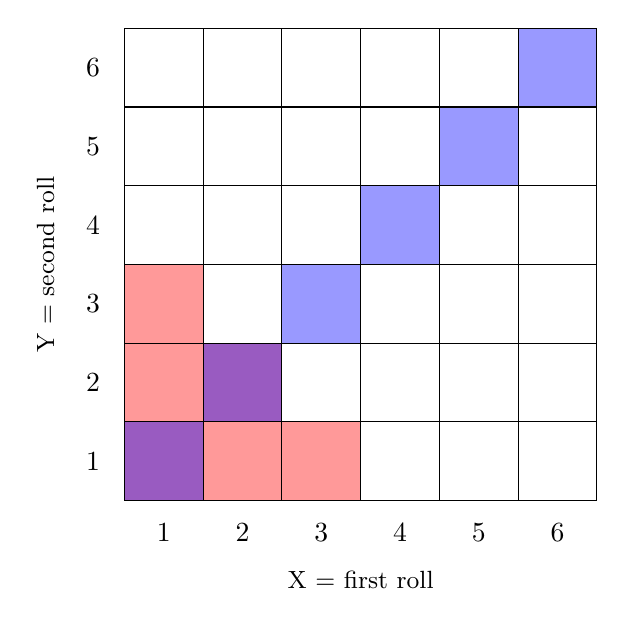
\begin{tikzpicture}
	\foreach \x in {1,...,3} {
		\fill[red!40] (0,\x-1) rectangle (4-\x,\x);
	}
	\foreach \x in {1,...,6} {
		\fill[blue,opacity=.4] (\x-1,\x-1) rectangle (\x,\x);
		\node at (\x-.5,-.4) {\x};
		\node at (-.4,\x-.5) {\x};
	}
	\draw (0,0) grid (6,6);
	\node at (3,-1) {\small X = first roll};
	\node[rotate=90] at (-1,3) {\small Y = second roll};
	\end{tikzpicture} \quad
	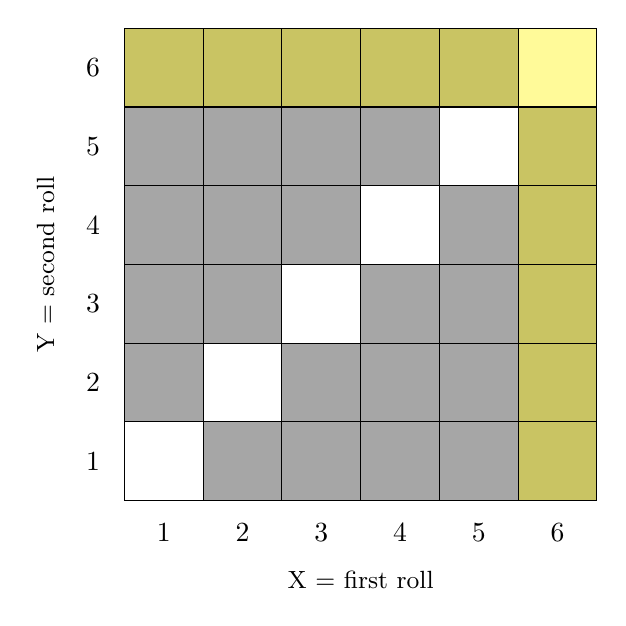
\begin{tikzpicture}
	\foreach \x in {1,...,6} {
		\fill[gray!70] (\x,\x-1) rectangle (6,\x);
		\fill[gray!70] (\x-1,\x) rectangle (\x,6);
		\node at (\x-.5,-.4) {\x};
		\node at (-.4,\x-.5) {\x};
	}
	\fill[yellow,opacity=.4] (0,5) rectangle (6,6);
	\fill[yellow,opacity=.4] (5,0) rectangle (6,5);
	\draw (0,0) grid (6,6);
	\node at (3,-1) {\small X = first roll};
	\node[rotate=90] at (-1,3) {\small Y = second roll};
	\end{tikzpicture}
\end{document} }
		\caption{On the left, the blue region shows the doubles and the red region
			indicates the outcomes whose sum is 4 or less; on the right, the yellow region
			indicates outcomes with at least one 6 and the gray region shows the outcomes
			where two rolls differ.}
		\label{fig:CondProbEx}
	\end{wrapfigure}
	
	Last summer, I taught myself \LaTeX\ and became a frequent user. I almost
	abandoned Microsoft Word completely since then and used \LaTeX\ whenever I found
	suitable. In fact, this file was typeset in \LuaLaTeX\ and source code can be
	found on \textit{GitHub}~\cite{Readmission}. I am able to typeset formulae like
	\begin{align*}
	\dd x \int_{t=\sin x}^{\tan x} e^{-t^2} \dt
		&= \dd x \paren{\int_{t=0}^{\tan x} e^{-t^2} \dt -
			\int_{t=0}^{\sin x} e^{-t^2} \dt} \\
		&= \dd x \int_{t=0}^{\tan x} e^{-t^2} \dt
			- \dd x \int_{t=0}^{\sin x} e^{-t^2} \dt \\
		&= e^{-\tan^2 x} \cdot \sec^2 x - e^{-\sin^2 x} \cdot \cos x.
	\end{align*}
	With the \TikZ\ package, I could make graphics like the figure on the right.
	Many standard computer tools (like \LaTeX\ and \textsc{gnu} toolchain) come as
	free and open source software (\textsc{foss}) and I came to know the underlying
	philosophy~\cite{free-sw} of it by this way. That is one of numerous benefits
	by studying computer science.
	
	That said, I did not find in computer science the same theoretical depth I
	found in mathematics and physics. Don't get me wrong. I did not mean all
	computer science and just most computer science curricula are not for
	theoretical computer scientists.
	
	I did not know that it is permissible and free to audit at a Chinese university
	until last fall. Hence I audited two courses at Fudan University, being
	\textit{mathematical analysis \Rn{1}} and \textit{advanced linear algebra
		\Rn{1}} respectively. I began to read some classics in mathematics like
	\textcite{BabyRudin} and \textcite{Zorich}. There were much discussion,
	especially between students and instructors. This actually motivates me to go
	back to Cornell to finish my study. True learning cannot happen without
	communication. And I think some important aspects of face-to-face communication
	cannot be replaced by virtual communication via the Internet. An academic
	environment is an integral part of any significant learning process.
	
	And I wish I could fulfill my curious and inquiring mind.
	
	\section*{Intended Major and Career Plan:}
	I intend to double major in mathematics and physics. I still love computer
	science and there is a lot more to learn in the field. But with the double
	major, I do not know if I have enough time and effort for it. In addition,
	there are general requirements to meet.
	
	If possible, I want to skip some lower division courses in mathematics and
	computer science like \textsc{mat} 122, \textsc{mat} 221, \textsc{csc} 140,
	\textsc{csc} 151. Due to my strong interest in mathematics, I will definitely
	have a wonderful time with mathematics. Since I do not have much background in
	physics, I will probably have a very hard time with it. But I like challenges;
	hard courses just turn me on and easy courses are time-wasters.
	
	I want to stay in the academia and become an academic (if not a mathematician).
	This means I will seek master and doctoral degrees after graduation from
	Cornell.

	\section*{Term I wish to return:}
	I wish to return on the block 1 of the 2016-2017 academic year.
	
	\section*{Housing Preference:}
	I do not have any particular housing preference, except that I want to make the
	habit of going to bed early.
	
	\clearpage
	
	\printbibliography
\end{document}